\documentclass[conference]{IEEEtran}
\IEEEoverridecommandlockouts
\usepackage{cite}
\usepackage{amsmath,amssymb,amsfonts}
\usepackage{graphicx}
\usepackage{booktabs}
\usepackage{textcomp}
\usepackage{xcolor}
\usepackage[hidelinks]{hyperref}
\usepackage{url}
\def\BibTeX{{\rm B\kern-.05em{\sc i\kern-.025em b}\kern-.08em
    T\kern-.1667em\lower.7ex\hbox{E}\kern-.125em\kern-.1667emX}}
\newcommand{\repo}{\url{https://github.com/dhruvo11/lumifuse-lowlight}}
\newcommand{\demo}{\url{https://lumifuse.streamlit.app}}

\begin{document}

\title{LumiFuse: Illumination-Adaptive Hybrid Low-Light Image Restoration Combining Retinex Priors with Zero-Reference Curve Estimation\\
\large Hackathon Problem P1 --- Team T81 (Bugweiser)}

\author{\IEEEauthorblockN{Dhruv S P}
\IEEEauthorblockA{USN: 1RUA24CSE0133\\
Team T81 (Bugweiser)}
\and
\IEEEauthorblockN{Harshit Rudresh}
\IEEEauthorblockA{USN: 1RUA24CSE0157\\
Team T81 (Bugweiser)}
}

\maketitle

\begin{abstract}
Images captured in low light are dark, noisy and colour-distorted, and any gain that lifts the shadows also amplifies
noise and clips regions that were already lit. We present \emph{LumiFuse}, an illumination-adaptive restoration
system that measures each image first and derives every parameter from those measurements. It runs two branches:
an adaptive classical pipeline (guided-filter Retinex decomposition, gain-aware edge-preserving denoising, adaptive
CLAHE and colour correction) and a 1.0\,M-parameter network built on Zero-DCE whose curve estimator and refinement
U-Net are conditioned on the classical illumination map and on a noise-amplification map. A reliability-weighted
fusion combines the branches per pixel, and no-reference quality gates correct exposure, residual noise and colour
cast. Trained on a de-duplicated, leak-free LOL split (we found that 89 of the 100 LOL-v2-real test images are
LOL-v1 training images), LumiFuse reaches 18.09\,dB PSNR / 0.7375 SSIM on LOL-v1 (+3.23\,dB over official Zero-DCE),
the best SSIM on four of five paired test sets, introduces no clipped pixels, and runs in 0.53\,s per
$600\times400$ frame on a laptop CPU. We report a 16-variant ablation, artefact metrics and an exposure-ambiguity
failure analysis. Code, weights and evaluation: \repo; live demo: \demo.
\end{abstract}

\begin{IEEEkeywords}
low-light image enhancement, Retinex, Zero-DCE, guided filter, CLAHE, hybrid restoration, image quality assessment
\end{IEEEkeywords}

\section{Introduction}
Low-light photography suffers from five coupled degradations: severe under-exposure, sensor noise, colour casts,
non-uniform illumination (lamps, windows, backlight) and loss of texture after denoising. Classical methods based
on Retinex theory~\cite{land1971retinex,jobson1997msrcr,guo2017lime} are fast and interpretable but use hand-set
parameters and amplify noise; learned enhancers~\cite{wei2018retinexnet,zhang2019kind,jiang2021enlightengan,
guo2020zerodce,cai2023retinexformer} restore better on their training distribution but are opaque and can fail on
unseen exposure levels. This work addresses the hackathon challenge of building an \emph{adaptive}, deployable
system that combines both and is evaluated honestly on unseen data. Our contributions are:
\begin{itemize}
\item An adaptive classical pipeline in which illumination smoothing, re-lighting exponent, denoising strength, CLAHE
clip limit and colour-correction strength are all computed from measured image statistics.
\item \emph{LumiNet}, a Zero-DCE~\cite{guo2020zerodce} curve estimator extended with a classical illumination-prior
channel plus a refinement U-Net conditioned on a classical noise-amplification map, fine-tuned from the official
weights.
\item A hybrid decision layer: two-sided input-exposure conditioning, reliability-weighted per-pixel fusion with a
brightness-dependent global trust term, and no-reference quality gates.
\item A leak-free protocol (test-overlap removal), evaluation on six test sets with all metrics requested by the
problem statement, a 16-variant ablation, artefact metrics, failure analysis, and a public web deployment.
\end{itemize}

\section{Related Work}
\textbf{Retinex and classical enhancement.} Retinex models an image as $I = R \odot L$~\cite{land1971retinex};
MSRCR~\cite{jobson1997msrcr} and LIME~\cite{guo2017lime} estimate and adjust the illumination $L$, LIME refining a
max-RGB initial map with a structure-aware prior. CLAHE~\cite{zuiderveld1994clahe} equalises local histograms with a
clip limit; bilateral~\cite{tomasi1998bilateral} and guided~\cite{he2013guided} filters smooth noise while keeping
edges. \textbf{Learned enhancement.} RetinexNet~\cite{wei2018retinexnet} introduced the paired LOL dataset and a
decomposition network; KinD~\cite{zhang2019kind} adds a dedicated denoising branch; EnlightenGAN~\cite{jiang2021enlightengan}
trains without pairs; Zero-DCE~\cite{guo2020zerodce} and Zero-DCE++~\cite{li2022zerodcepp} estimate pixel-wise
quadratic curves with zero-reference losses; Retinexformer~\cite{cai2023retinexformer} is a recent transformer.
LumiFuse keeps the efficiency and monotonicity of curve estimation and injects classical priors where curves are
weakest: noise and colour.

\section{Method}
Fig.~\ref{fig:arch} shows the inference path; module and function names in the figure match the repository.

\begin{figure*}[t]
\centering
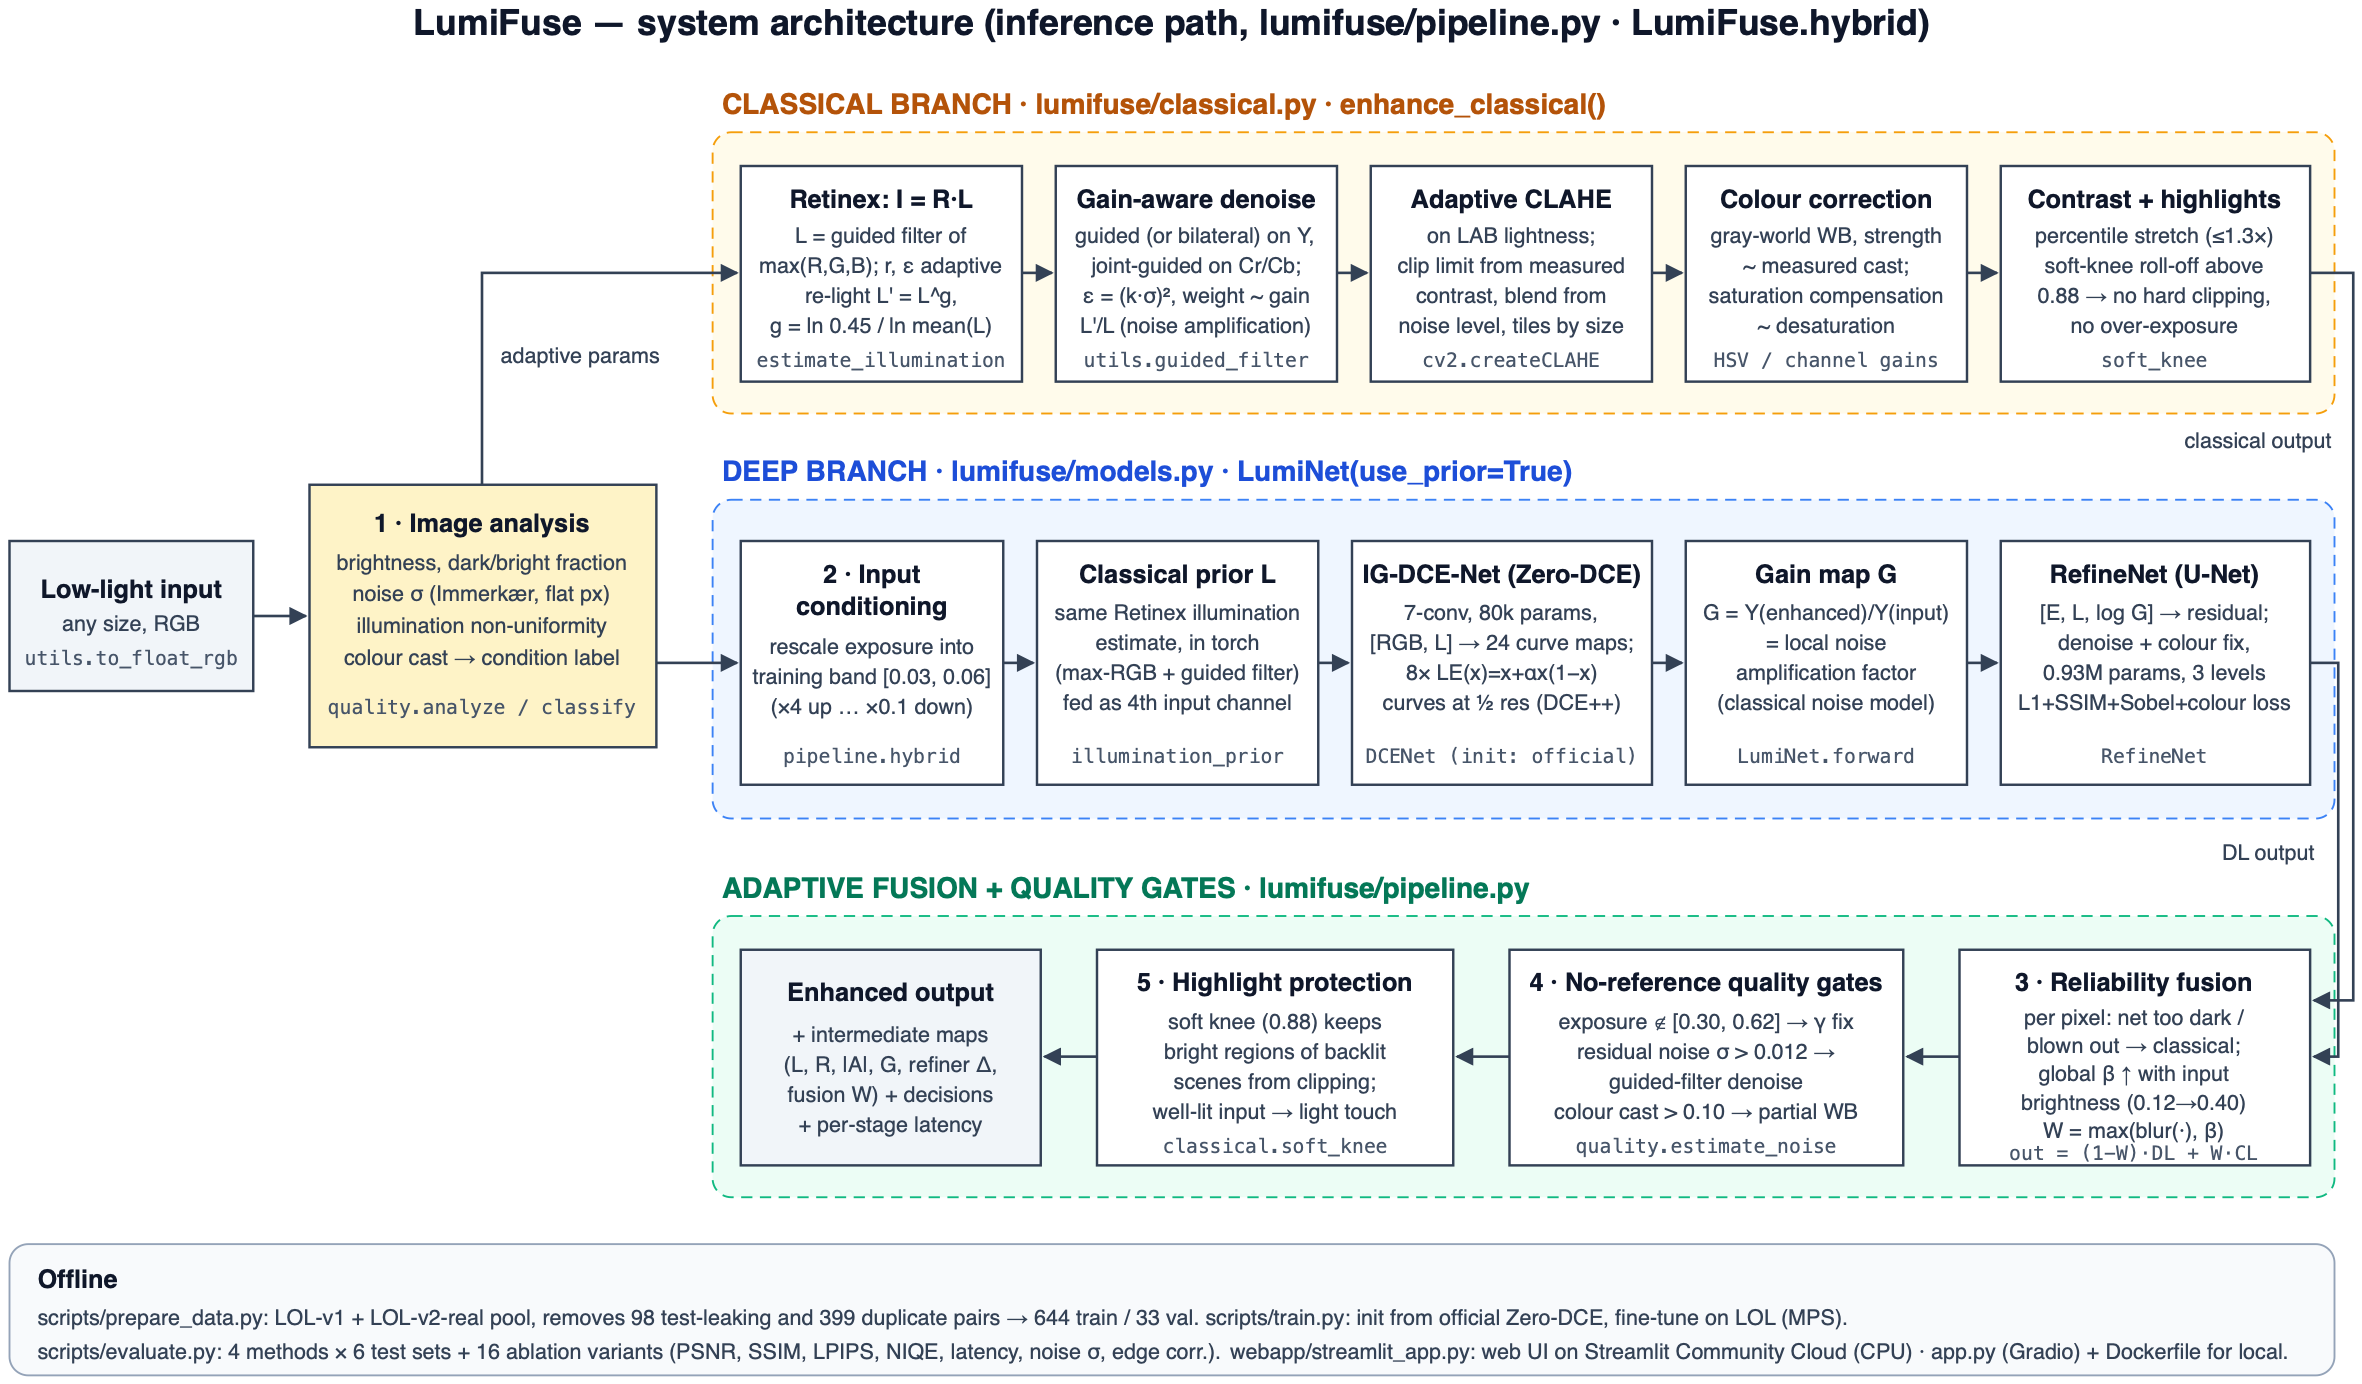
\includegraphics[width=\textwidth]{figures/architecture.png}
\caption{LumiFuse architecture. An analysis stage measures the input; a classical branch (top) and an
illumination-guided deep branch (middle) restore it in parallel; reliability fusion and no-reference quality gates
(bottom) produce the output together with all intermediate maps.}
\label{fig:arch}
\end{figure*}

\subsection{Image analysis}
For each input we measure mean/median luminance, the fraction of dark ($Y<0.1$) and bright ($Y>0.85$) pixels,
illumination non-uniformity (standard deviation of the log of a heavily blurred max-RGB map), colour cast
$(\max_c\mu_c-\min_c\mu_c)/\bar\mu$, and the noise standard deviation $\sigma$ with Immerk{\ae}r's
operator~\cite{immerkaer1996noise} restricted to the flattest 50\,\% of pixels so that texture is not counted as
noise. These values select every parameter below and a condition label shown to the user.

\subsection{Adaptive classical branch}
\textbf{Illumination and re-lighting.} $L_0=\max_c I_c$ is refined by a self-guided filter $L=\mathrm{GF}(L_0,L_0;r,\epsilon)$
with $r=\min(H,W)/50$ and $\epsilon=(0.1\,P_{90}(L_0))^2$, which makes the smoothing scale-invariant to exposure. The
illumination is re-lit as $L'=L^{g}$ and the image as $\hat I = I\odot L'/L$, with
\begin{equation}
g=\mathrm{clip}\!\left(\frac{\ln 0.45}{\ln \exp(\overline{\ln L})},\,0.15,\,1\right),
\end{equation}
mapping the log-average illumination to the brightness of well-exposed references. Because $L'/L=L^{g-1}$, dark
regions are lifted most and regions with $L\approx1$ are left unchanged, which protects highlights.
\textbf{Gain-aware denoising.} After re-lighting, $\sigma$ is re-measured; luma is filtered by a guided filter with
$\epsilon_Y=(5\sigma)^2$ (bilateral is selectable) and chroma by a joint guided filter guided by the clean luma. The
filtered result is blended per pixel with weight $\propto (L'/L)$, so noise suppression follows amplification.
\textbf{CLAHE} is applied to LAB lightness with clip limit $1+2.5(0.22-c)/0.22\in[1,3]$ from the RMS contrast $c$
and a lighter blend for noisy images. \textbf{Colour correction} applies gray-world gains with strength proportional
to the measured cast, and saturation compensation proportional to the measured desaturation. A percentile contrast
stretch (skipped when $\sigma>0.02$) and a soft-knee roll-off above 0.88 complete the branch. With
\texttt{adaptive=False} each rule is replaced by a fixed constant.

\subsection{Illumination-guided deep branch (LumiNet)}
\textbf{Curve stage.} The Zero-DCE estimator (seven $3\times3$ convolutions, 32 channels) receives $[I, L]$, where $L$
is the same guided-filter illumination computed in PyTorch, and predicts eight three-channel curve maps $A_n$ applied
iteratively:
\begin{equation}
E_n = E_{n-1} + A_n \odot E_{n-1}\odot(1-E_{n-1}),\quad E_0=I .
\end{equation}
Curves are estimated at half resolution and bilinearly up-sampled as in Zero-DCE++~\cite{li2022zerodcepp}. The
network is initialised from the authors' weights; the new input channel is zero-initialised, so training starts
exactly at official Zero-DCE. \textbf{Refinement.} Curves can brighten but cannot denoise. A three-level
U-Net~\cite{ronneberger2015unet} (0.93\,M parameters) receives $[E, L, \tfrac14\log G]$ with the amplification map
$G=Y(E)/(Y(I)+0.02)$---a classical noise model telling the network how much each pixel's noise was multiplied---and
predicts a residual: $\hat Y = E + \mathcal{R}_\theta(E,L,G)$.
\textbf{Losses.} The refiner is trained with $\mathcal{L}_1+0.2(1-\mathrm{SSIM})+0.1\,\mathcal{L}_1(\nabla_{\!S})
+0.1\,\mathcal{L}_{\angle}$, where $\nabla_{\!S}$ are Sobel gradients (edge preservation) and $\mathcal{L}_{\angle}$
is the cosine distance between RGB vectors (colour shifts). The curve stage is trained with a low-pass
$\mathcal{L}_1$ ($4\times4$ average pooling, since curves should not chase noise), $0.5\,\mathcal{L}_{\angle}$, and the
Zero-DCE illumination-smoothness term $10\,\mathrm{TV}(A)$. The curve output is detached before the refiner; without
this, joint optimisation collapsed the curve stage into a feature map (mean R/G outputs 0.07/0.92).

\subsection{Hybrid decision layer}
\textbf{Input conditioning.} The network learned the exposure mapping of LOL inputs (mean luminance $\mu_0=0.05$).
Inputs outside $[0.6\mu_0, 1.2\mu_0]$ are rescaled by $k=\mu_0/\mu$ (at most $4\times$) or $k=1.2\mu_0/\mu$
(at least $0.1\times$). \textbf{Reliability fusion.} With $Y_D$, $Y_C$ the luminance of the deep and classical
outputs, $u=\mathrm{clip}((0.12-Y_D)/0.12)\,[Y_C>Y_D]$ marks regions left too dark and
$o=\mathrm{clip}((Y_D-0.9)/0.1)\,[Y_C<Y_D]$ regions blown out; a global trust term
$\beta=\mathrm{clip}((\mu-0.12)/(0.40-0.12),0,0.9)$ shifts weight to the classical branch for moderately dark inputs,
where the network's strong denoising flattens contrast. Then
\begin{equation}
W=\max\!\big(\mathcal{G}_{s}(\max(u,o)),\,\beta\big),\qquad \hat I=(1-W)\odot D + W\odot C,
\end{equation}
with a Gaussian blur $\mathcal{G}_s$, $s=\min(H,W)/80$, to avoid seams. \textbf{Quality gates.} If the mean output
luminance leaves $[0.30,0.62]$ a luminance-only gamma restores it; if residual $\sigma>0.012$ a guided-filter
denoise is applied; if the colour cast exceeds 0.10 a partial gray-world correction is applied; a soft knee
protects highlights. Well-lit inputs ($\mu>0.35$) are blended back towards the original.

\section{Experimental Setup}
\textbf{Data and leak-free split.} We pooled LOL-v1 \texttt{our485}~\cite{wei2018retinexnet} and LOL-v2-real
\texttt{Train}~\cite{yang2021lolv2}. Hashing every low-light input revealed that 89 of the 100 LOL-v2-real test
images are pixel-identical to LOL-v1 training images. We removed all 98 pairs overlapping either test set and 399
duplicates, leaving 644 training and 33 validation pairs. The validation split---never the test sets---was used for
checkpoint selection and every hyper-parameter, including synthetic variants of validation images for exposure
thresholds. \textbf{Test sets.} LOL-v1 \texttt{eval15}; LOL-v2-real test (100); three synthetic conditions built from
30 unseen LOL-v2 references with a Poisson--Gaussian camera model~\cite{foi2008noise} (linearise, scale exposure,
shot + read noise, re-encode, 8-bit quantise): moderate ($\times0.08$--$0.15$), extreme-dark
($\times0.003$--$0.006$) and non-uniform (gradient + spotlight, $\times0.004$--$0.6$); and 74 real DICM~\cite{lee2013dicm}
and LIME~\cite{guo2017lime} photographs. \textbf{Metrics} (in the order of the problem statement): PSNR and
SSIM~\cite{wang2004ssim} on RGB; LPIPS (AlexNet)~\cite{zhang2018lpips}; NIQE~\cite{mittal2013niqe} (MATLAB-equivalent
implementation); CPU latency; residual noise $\sigma$; edge preservation (correlation of Sobel magnitudes with the
reference). No ground-truth-mean brightness correction is applied to any score. \textbf{Training.} 4000 iterations,
batch 8, $160^2$ crops with flips/rotations and illumination augmentation (30\,\% darkened $\times0.3$--1, 15\,\%
brightened $\times1$--2, 20\,\% multiplied by a random smooth field), AdamW with one-cycle schedule ($4\times10^{-4}$
refiner, $2\times10^{-4}$ curve stage), Apple M1 GPU, about 40 minutes per model. The DL-only baseline is the
same network and recipe without the prior channels.

\section{Results}
\begin{table*}[t]
\centering
\caption{Comparison of classical, deep-learning and hybrid approaches on the paired LOL benchmarks (best in bold). LOL-v2-real test images never appear in training. Latency: Apple M1 CPU, 4 threads, $600\times400$ input.}
\label{tab:main}
\setlength{\tabcolsep}{5pt}
\begin{tabular}{l cccc cccc c}
\toprule
 & \multicolumn{4}{c}{LOL-v1 eval15 (15 images)} & \multicolumn{4}{c}{LOL-v2-real test (100 images)} & \\
\cmidrule(lr){2-5}\cmidrule(lr){6-9}
Method & PSNR$\uparrow$ & SSIM$\uparrow$ & LPIPS$\downarrow$ & NIQE$\downarrow$ & PSNR$\uparrow$ & SSIM$\uparrow$ & LPIPS$\downarrow$ & NIQE$\downarrow$ & ms/frame \\
\midrule
Classical (adaptive) & 17.06 & 0.6612 & 0.386 & 6.42 & \textbf{19.12} & 0.6890 & 0.399 & 6.58 & 64 \\
Zero-DCE (official) & 14.86 & 0.5627 & 0.335 & 7.65 & 18.06 & 0.5798 & 0.312 & 7.90 & 276 \\
DL-only (LumiNet, no priors) & 17.23 & 0.7344 & \textbf{0.270} & \textbf{3.86} & 16.14 & \textbf{0.7382} & \textbf{0.296} & \textbf{3.96} & 308 \\
\textbf{LumiFuse (hybrid)} & \textbf{18.09} & \textbf{0.7375} & 0.318 & 4.87 & 17.41 & 0.7378 & 0.354 & 4.72 & 529 \\
\bottomrule
\end{tabular}
\end{table*}


\textbf{Benchmark comparison.} Table~\ref{tab:main} compares the four approaches. Our official Zero-DCE result on
LOL-v1 (14.86\,dB) reproduces the value reported in~\cite{guo2020zerodce}, validating the metric code. LumiFuse
obtains the best PSNR and SSIM on LOL-v1 (18.09\,dB / 0.7375; +3.23\,dB over Zero-DCE, +1.03\,dB over the classical
pipeline, +0.86\,dB over DL-only). On LOL-v2 it ties DL-only on SSIM but its PSNR is below the classical pipeline;
Section~\ref{sec:failure} shows that this is a global-exposure choice rather than restoration error. DL-only has the
best LPIPS and NIQE: the classical priors push the refiner towards stronger denoising, which raises fidelity at some
cost in texture---the perception--distortion trade-off~\cite{blau2018perception}. Fig.~\ref{fig:lol} shows examples.

\begin{figure*}[t]
\centering
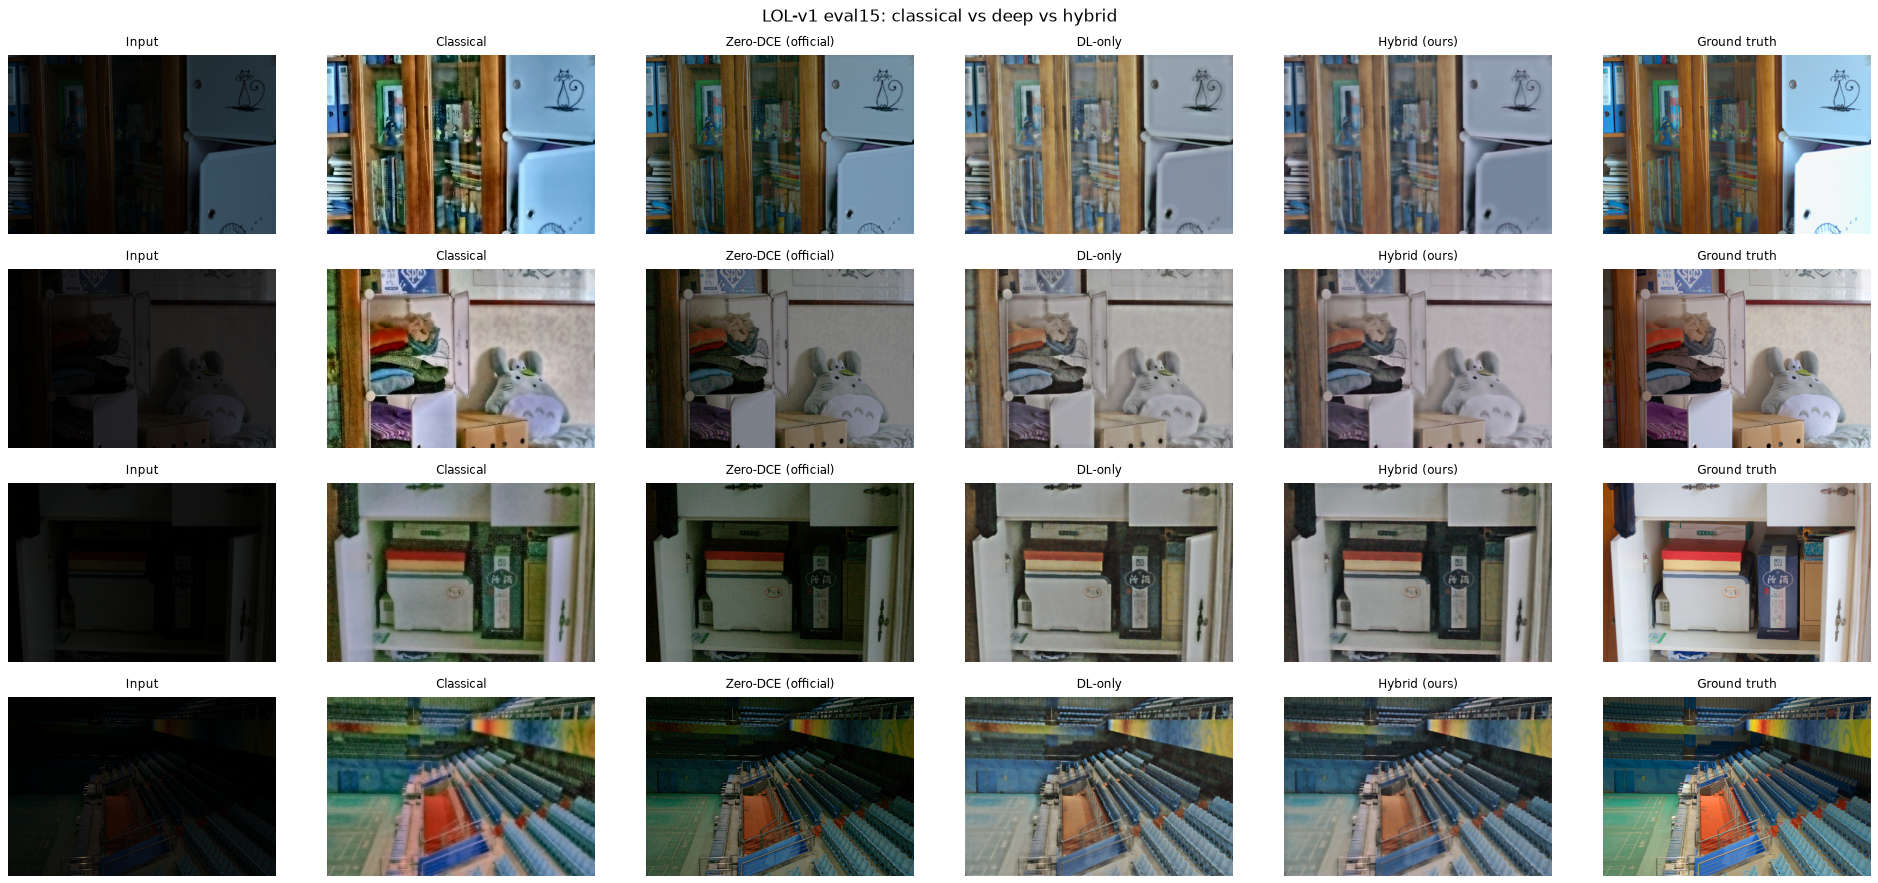
\includegraphics[width=\textwidth]{figures/comparison_lol.png}
\caption{LOL-v1 examples. Classical output is grainy, official Zero-DCE is washed out with colour casts, DL-only is
clean but flat; LumiFuse balances exposure, noise and colour.}
\label{fig:lol}
\end{figure*}

\begin{table*}[t]
\centering
\caption{Generalisation across illumination conditions on unseen scenes: synthetic moderate, extremely dark and non-uniform (gradient + spotlight) lighting built from 30 LOL-v2 test references with a Poisson--Gaussian camera model, and 74 real DICM/LIME photographs (no reference, NIQE).}
\label{tab:conditions}
\setlength{\tabcolsep}{5pt}
\begin{tabular}{l ccc ccc ccc c}
\toprule
 & \multicolumn{3}{c}{Moderate ($\times$0.08--0.15)} & \multicolumn{3}{c}{Extreme-dark ($\times$0.003--0.006)} & \multicolumn{3}{c}{Non-uniform} & Real \\
\cmidrule(lr){2-4}\cmidrule(lr){5-7}\cmidrule(lr){8-10}\cmidrule(lr){11-11}
Method & PSNR & SSIM & LPIPS & PSNR & SSIM & LPIPS & PSNR & SSIM & LPIPS & NIQE \\
\midrule
Classical (adaptive) & 17.87 & 0.762 & 0.254 & 14.99 & 0.317 & 0.908 & \textbf{16.88} & 0.748 & 0.266 & 3.86 \\
Zero-DCE (official) & \textbf{18.50} & 0.738 & \textbf{0.245} & 10.34 & 0.083 & 1.300 & 16.82 & 0.720 & 0.274 & \textbf{3.80} \\
DL-only (LumiNet, no priors) & 13.53 & 0.737 & 0.314 & 15.78 & 0.490 & \textbf{0.746} & 13.94 & 0.738 & 0.322 & 3.94 \\
\textbf{LumiFuse (hybrid)} & 17.10 & \textbf{0.799} & 0.262 & \textbf{16.01} & \textbf{0.501} & 0.763 & 16.73 & \textbf{0.796} & \textbf{0.252} & 4.13 \\
\bottomrule
\end{tabular}
\end{table*}


\textbf{Generalisation across illumination.} Table~\ref{tab:conditions} and Figs.~\ref{fig:syn}--\ref{fig:real}
evaluate unseen lighting conditions. On extremely dark inputs LumiFuse is best on PSNR and SSIM (16.01\,dB / 0.501
versus 0.317 classical and 0.083 Zero-DCE). Under moderate and non-uniform light it has the best SSIM (0.799 and
0.796) while the classical pipeline or Zero-DCE keep slightly higher PSNR. On real photographs the classical and
Zero-DCE outputs have marginally lower NIQE (3.80--3.86 vs.\ 4.13); NIQE rewards high-frequency texture, including
residual noise.

\begin{figure*}[t]
\centering
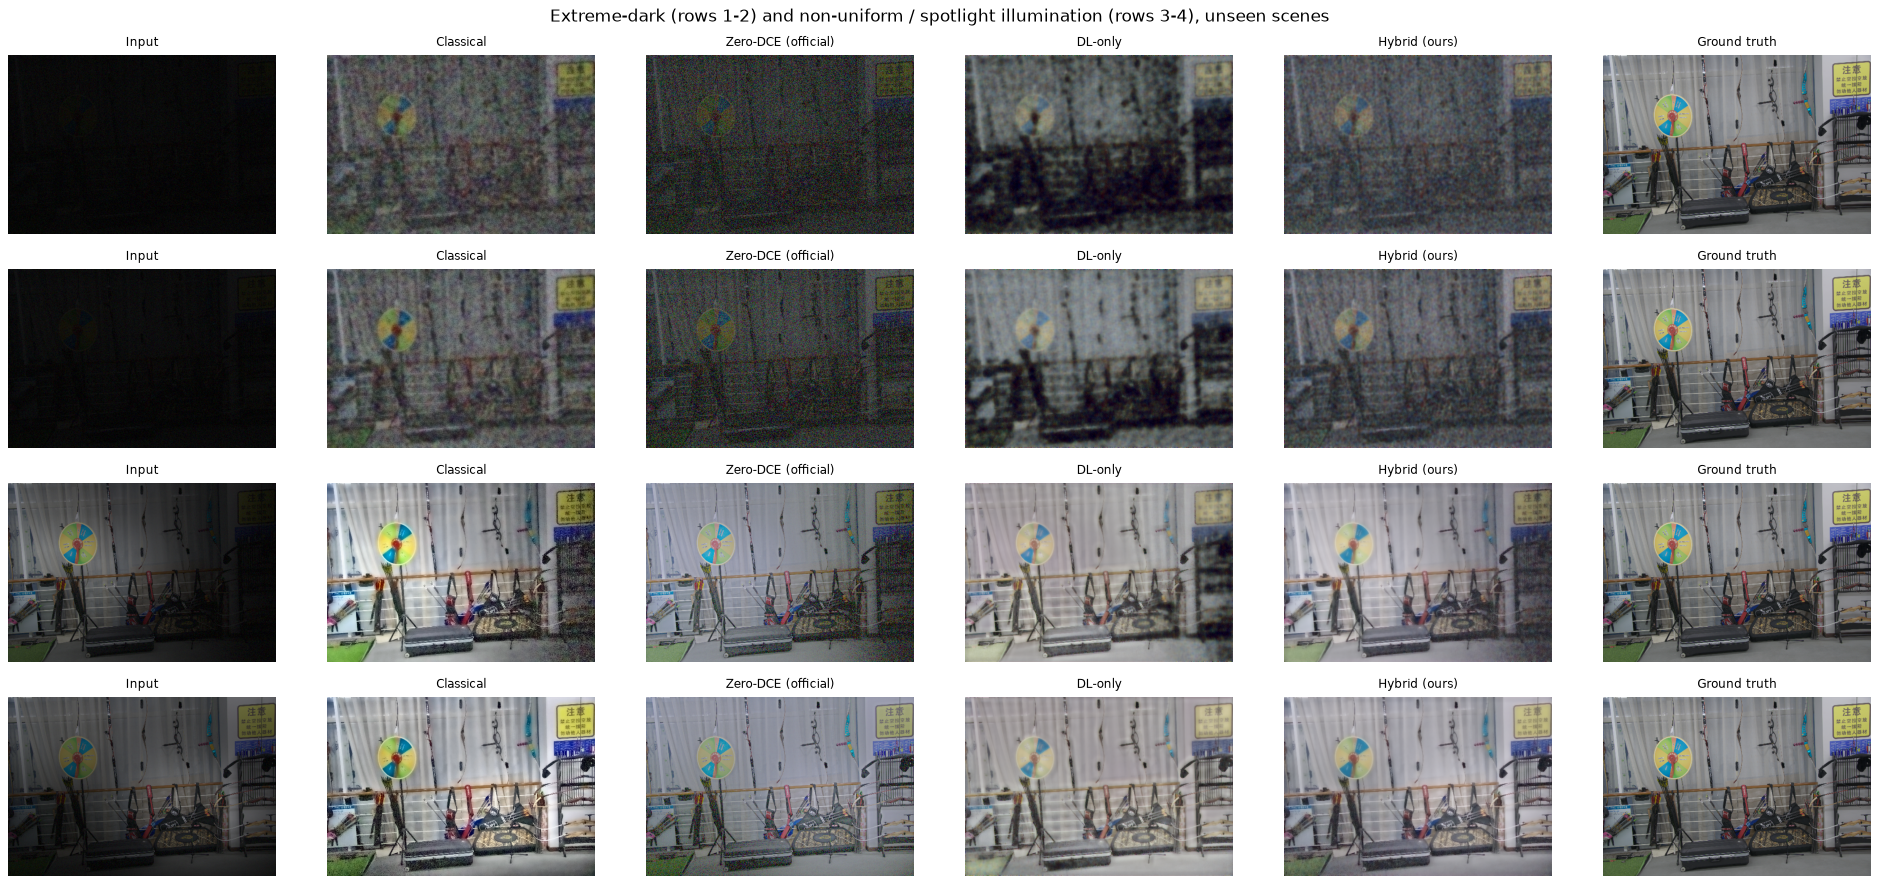
\includegraphics[width=\textwidth]{figures/conditions_synthetic.png}
\caption{Unseen scenes under extreme darkness (rows 1--2) and non-uniform spotlight illumination (rows 3--4).}
\label{fig:syn}
\end{figure*}

\begin{figure}[t]
\centering
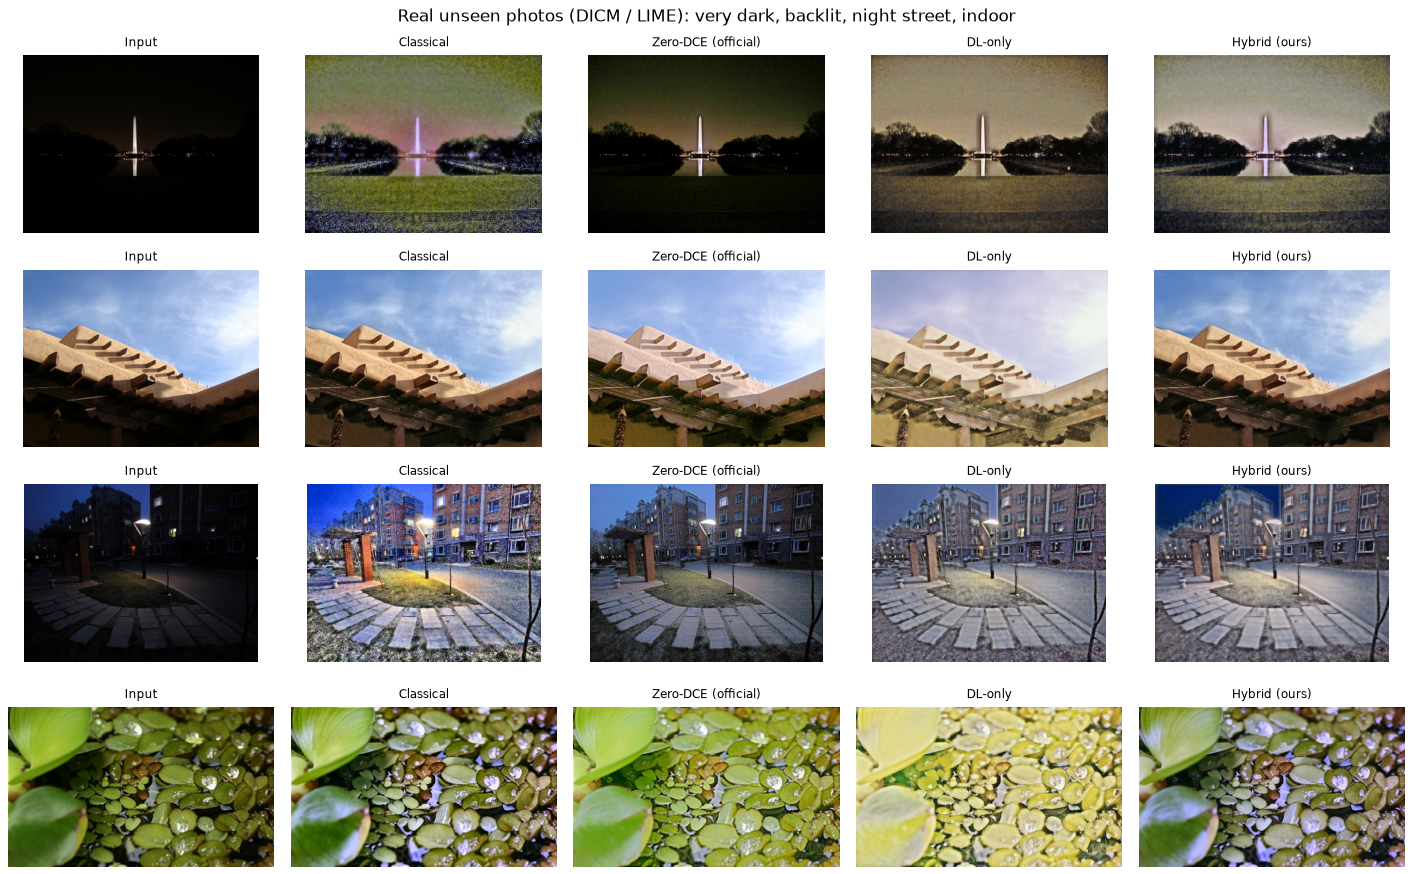
\includegraphics[width=\columnwidth]{figures/conditions_real.png}
\caption{Real photographs (DICM/LIME): very dark, backlit, night street and indoor scenes.}
\label{fig:real}
\end{figure}

\begin{table}[t]
\centering
\caption{Artefacts: newly clipped pixels (\%), colour shift (CIEDE2000 $\Delta E$, RGB angle in degrees), edge preservation (Sobel-magnitude correlation) and residual noise $\sigma$.}
\label{tab:artifacts}
\setlength{\tabcolsep}{3pt}
\footnotesize
\begin{tabular}{l ccccc}
\toprule
Method & Clip\%$\downarrow$ & $\Delta E\downarrow$ & Angle$\downarrow$ & Edge$\uparrow$ & Noise $\sigma\downarrow$ \\
\midrule
\multicolumn{6}{l}{\textit{LOL-v2-real test}}\\
Classical & 0.004 & \textbf{12.8} & 7.6 & 0.777 & 0.0151 \\
Zero-DCE & 0.000 & 14.2 & 12.4 & \textbf{0.882} & 0.0215 \\
DL-only & 0.000 & 15.4 & \textbf{4.1} & 0.839 & 0.0032 \\
\textbf{LumiFuse} & \textbf{0.000} & 13.5 & 4.3 & 0.792 & \textbf{0.0024} \\
\midrule
\multicolumn{6}{l}{\textit{Synthetic extreme-dark}}\\
Classical & \textbf{0.000} & 16.0 & \textbf{4.2} & 0.192 & 0.0402 \\
Zero-DCE & 0.000 & 30.4 & 29.2 & 0.141 & 0.0910 \\
DL-only & 0.000 & \textbf{15.7} & 7.7 & 0.372 & 0.0088 \\
\textbf{LumiFuse} & 0.000 & 16.2 & 5.8 & \textbf{0.385} & \textbf{0.0074} \\
\bottomrule
\end{tabular}
\end{table}


\textbf{Over-exposure, colour shift and detail loss.} Table~\ref{tab:artifacts} quantifies the artefacts named in
the challenge. LumiFuse introduces no clipped pixels on any test set (the curve formulation cannot exceed 1 and the
soft knee rolls off highlights), whereas the classical stretch clips up to 0.11\,\% on LOL-v1. Its hue error is
close to the best on LOL-v2 and much lower than Zero-DCE on extreme-dark inputs (5.8$^\circ$ vs.\ 29.2$^\circ$),
and it preserves the most edge structure there. $\Delta E$ also counts brightness and therefore mirrors the
exposure differences discussed below.

\textbf{Intermediate representations.} Fig.~\ref{fig:inter} shows the maps the system exposes: the classical
illumination prior, reflectance, curve strength, curve-stage output, amplification map $G$, refiner correction,
classical output and fusion weights. The refiner correction is largest exactly where $G$ is large, confirming that
the network uses the noise-amplification prior.

\begin{figure*}[t]
\centering
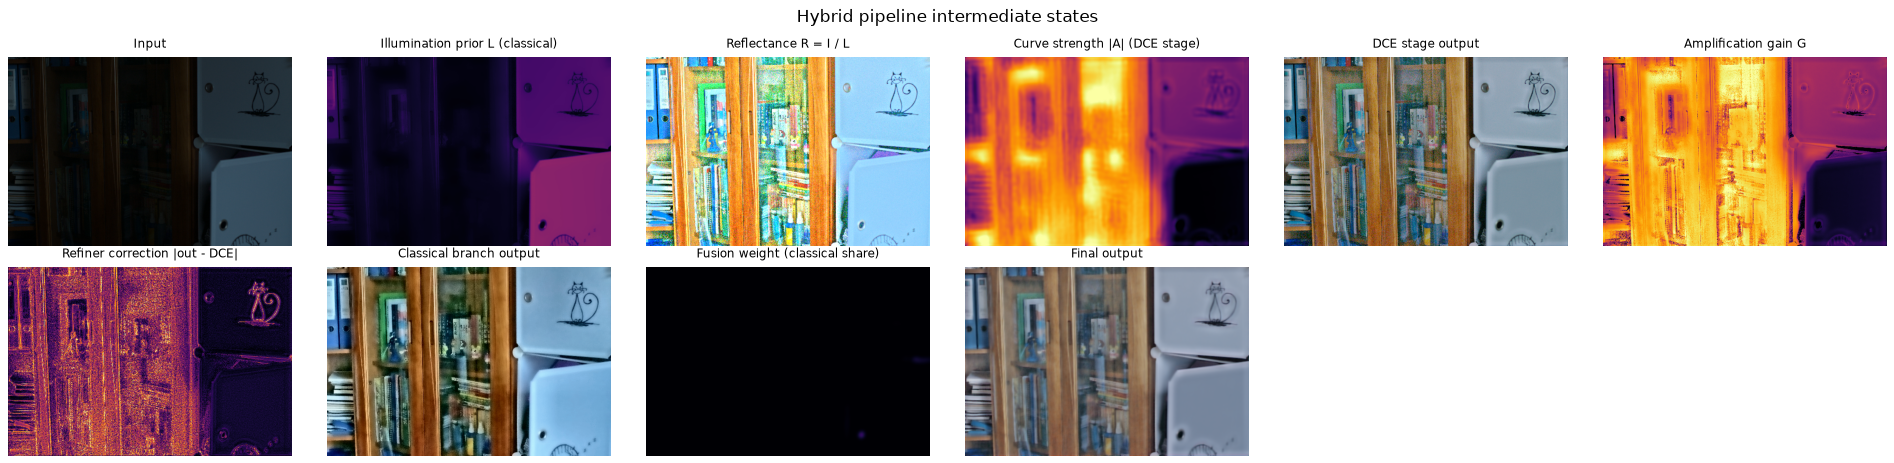
\includegraphics[width=\textwidth]{figures/intermediates_lol.png}
\caption{Intermediate states of the hybrid pipeline for a LOL-v1 input.}
\label{fig:inter}
\end{figure*}

\begin{table*}[t]
\centering
\caption{Ablation of the hybrid system: each row removes one component (PSNR / SSIM; best in bold).}
\label{tab:ablation}
\setlength{\tabcolsep}{6pt}
\begin{tabular}{l cc cc cc cc}
\toprule
 & \multicolumn{2}{c}{LOL-v1} & \multicolumn{2}{c}{LOL-v2-real} & \multicolumn{2}{c}{Extreme-dark} & \multicolumn{2}{c}{Non-uniform} \\
\cmidrule(lr){2-3}\cmidrule(lr){4-5}\cmidrule(lr){6-7}\cmidrule(lr){8-9}
Variant & PSNR & SSIM & PSNR & SSIM & PSNR & SSIM & PSNR & SSIM \\
\midrule
Full LumiFuse & 18.09 & 0.737 & 17.41 & 0.738 & 16.01 & 0.501 & 16.73 & 0.796 \\
$-$ classical priors ($L$, $G$) & 17.09 & 0.735 & 16.27 & 0.737 & 16.80 & 0.530 & \textbf{16.96} & \textbf{0.803} \\
$-$ RefineNet & 18.08 & 0.714 & 16.85 & 0.725 & \textbf{17.33} & 0.513 & 16.25 & 0.748 \\
$-$ LOL fine-tuning & 15.06 & 0.700 & \textbf{20.02} & \textbf{0.776} & 14.01 & \textbf{0.530} & 16.91 & 0.791 \\
$-$ input conditioning & 18.10 & 0.736 & 17.24 & 0.735 & 15.95 & 0.501 & 14.98 & 0.762 \\
$-$ reliability fusion & 18.09 & 0.737 & 17.40 & 0.737 & 16.01 & 0.501 & 15.64 & 0.742 \\
$-$ global trust $\beta$ & 18.09 & 0.737 & 17.40 & 0.737 & 16.01 & 0.501 & 15.64 & 0.742 \\
$-$ quality gates & \textbf{18.13} & \textbf{0.738} & 17.27 & 0.738 & 15.71 & 0.501 & 16.73 & 0.796 \\
$-$ highlight protection & 18.09 & 0.737 & 17.41 & 0.738 & 16.01 & 0.501 & 16.73 & 0.796 \\
\bottomrule
\end{tabular}
\end{table*}


\textbf{Ablation.} Table~\ref{tab:ablation} removes one component at a time. The classical priors add +1.00\,dB on
LOL-v1 and +1.14\,dB on LOL-v2 (on the synthetic sets the prior-free network is slightly better, and it always has
better LPIPS/NIQE). Removing the refiner leaves LOL-v1 PSNR unchanged but lowers SSIM by 0.023--0.049 and triples
residual noise. Fine-tuning adds +3.03\,dB on LOL-v1 and +2.0\,dB on extreme-dark but costs 2.6\,dB on LOL-v2,
whose references are darker. Input conditioning (+1.75\,dB) and the global trust term (+1.09\,dB, SSIM +0.054)
matter most under non-uniform light; the per-pixel reliability map rarely fires on these sets and acts as a safety
net for blown highlights in real photos. Quality gates add +0.30\,dB on extreme-dark and +0.14\,dB on LOL-v2.

\begin{table}[t]
\centering
\caption{Ablation of the classical pipeline (PSNR / SSIM).}
\label{tab:classical}
\setlength{\tabcolsep}{2.5pt}
\footnotesize
\begin{tabular}{l cc cc cc}
\toprule
 & \multicolumn{2}{c}{LOL-v1} & \multicolumn{2}{c}{LOL-v2} & \multicolumn{2}{c}{Extreme} \\
\cmidrule(lr){2-3}\cmidrule(lr){4-5}\cmidrule(lr){6-7}
Variant & PSNR & SSIM & PSNR & SSIM & PSNR & SSIM \\
\midrule
Adaptive, full & 17.06 & 0.661 & 19.12 & 0.689 & 14.99 & 0.317 \\
Fixed parameters & 15.27 & 0.639 & 17.64 & 0.639 & 12.79 & 0.115 \\
$-$ Retinex & 9.24 & 0.345 & 11.40 & 0.355 & 7.55 & 0.150 \\
$-$ denoising & 15.90 & 0.374 & 16.67 & 0.401 & 11.69 & 0.074 \\
Bilateral (vs guided) & 16.74 & 0.590 & 18.38 & 0.607 & 14.82 & 0.216 \\
$-$ CLAHE & \textbf{17.17} & \textbf{0.707} & \textbf{20.24} & \textbf{0.736} & 13.25 & \textbf{0.466} \\
$-$ colour correction & 17.11 & 0.665 & 18.47 & 0.689 & \textbf{15.16} & 0.319 \\
\bottomrule
\end{tabular}
\end{table}


Table~\ref{tab:classical} ablates the classical branch. Retinex re-lighting is essential ($-7.8$\,dB without it);
denoising adds 1.2--3.3\,dB; guided filtering beats bilateral filtering; adaptive parameters beat fixed ones by
+1.79\,dB (LOL-v1), +1.48\,dB (LOL-v2) and +2.20\,dB (extreme-dark). CLAHE, required by the challenge, lowers PSNR
against the low-contrast LOL references while increasing local contrast; we therefore use an adaptive clip limit
and a noise-dependent blend.

\section{Failure Analysis and Limitations}
\label{sec:failure}
\begin{table}[t]
\centering
\caption{Exposure diagnostic: PSNR before and after rescaling each output's mean brightness to the reference (GT-mean; diagnostic only, never reported as a score). Bold: best GT-mean PSNR over all four methods. Last column: hybrid mean absolute brightness error.}
\label{tab:exposure}
\setlength{\tabcolsep}{3pt}
\footnotesize
\begin{tabular}{l cc cc c}
\toprule
 & \multicolumn{2}{c}{Classical} & \multicolumn{2}{c}{LumiFuse} & \\
\cmidrule(lr){2-3}\cmidrule(lr){4-5}
Set & PSNR & GT-mean & PSNR & GT-mean & $|\Delta Y|$ \\
\midrule
LOL-v1 & 17.06 & 19.65 & 18.09 & 20.98 & 0.081 \\
LOL-v2 & 19.12 & 21.27 & 17.41 & \textbf{22.30} & 0.102 \\
Moderate & 17.87 & \textbf{20.06} & 17.10 & 20.06 & 0.094 \\
Extreme & 14.99 & 18.85 & 16.01 & \textbf{21.00} & 0.123 \\
Non-unif. & 16.88 & 18.23 & 16.73 & \textbf{18.94} & 0.078 \\
\bottomrule
\end{tabular}
\end{table}


\textbf{Global exposure ambiguity.} On a few LOL-v2 scene series (e.g.\ \texttt{00724}--\texttt{00730},
\texttt{00763}--\texttt{00764}) LumiFuse produces a mean brightness near 0.5 where the reference is near 0.33,
losing up to $\sim$10\,dB on those images (Fig.~\ref{fig:fail}). Rescaling each output's mean brightness to the
reference (a diagnostic that uses the ground truth and is never reported as a score) lifts LumiFuse to the best
value on LOL-v2 (22.30\,dB vs.\ 21.27\,dB for the classical pipeline) and on every other paired set except moderate
light, where it ties (Table~\ref{tab:exposure}). The deficit is therefore exposure choice, not restoration quality.
Target brightness is ill-posed from a dark input: references use photographer-chosen exposures, the network learns
their average, and PSNR penalises a global offset heavily (a uniform error of 0.1 alone caps PSNR at 20\,dB). Using
the classical illumination estimate as the exposure target lowered validation PSNR from 18.54 to 17.39\,dB and was
rejected. Mitigations: a user-controlled target exposure (Zero-DCE's exposure loss already takes a target) or
exposure-conditioned training.

\begin{figure}[t]
\centering
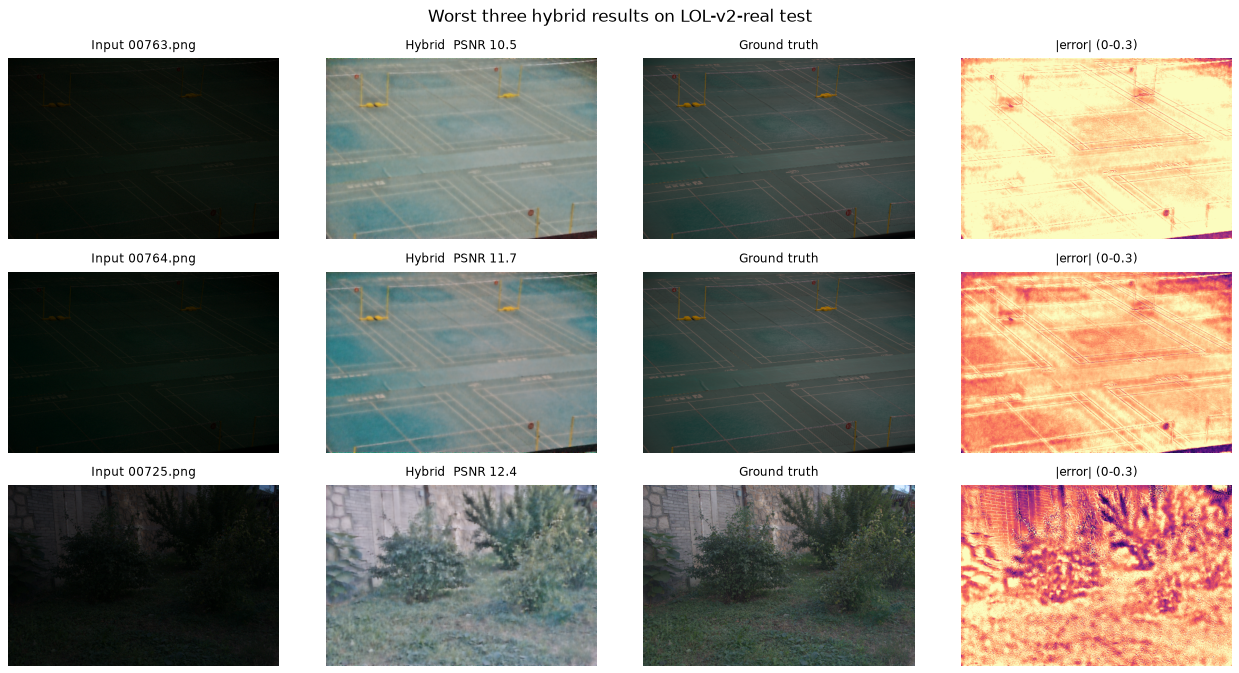
\includegraphics[width=\columnwidth]{figures/failure_cases.png}
\caption{Worst LumiFuse results on LOL-v2-real: output, reference and absolute error. Errors are dominated by global
brightness.}
\label{fig:fail}
\end{figure}

\textbf{Extreme darkness.} At $\times0.003$ exposure a white surface collects tens of photons and the shadows occupy
1--5 code values after 8-bit quantisation; every method has low SSIM there and LumiFuse leaves low-frequency chroma
blotches. RAW or burst input and refiner training with synthetic Poisson--Gaussian noise are the natural fixes.
\textbf{Other limitations.} The classical re-lighting exponent is global, so a bright spotlight reduces the lift of
the dark side; strong point lights in real photographs show amplified lens glare; training data are mostly indoor
LOL scenes. \textbf{Ethics.} The refiner is a learned prior that can smooth or, rarely, invent fine texture, so
outputs must not be used as forensic or medical evidence. The web application processes images in memory and stores
nothing. Datasets are used under their research terms and are not redistributed.

\section{Deployment and Reproducibility}
The system is deployed as a Streamlit web application on Streamlit Community Cloud (\demo) with a before/after
slider, intermediate maps, a compare-all mode, PNG download and explicit error states; inputs are capped at 768\,px
and a photo is processed in about 1.6\,s on the cloud CPU. A Gradio version and a Dockerfile (built and run, 1.7\,s
per request in the container) provide one-command local use, and \texttt{run\_inference.py} provides batch
inference. The repository (\repo) contains all source code, trained weights, the architecture diagram, a design
document, the evaluation file \texttt{eval\_P1\_T81.md}, ablation and failure analyses and 23 robustness tests. A
fresh clone that re-downloads all datasets and re-runs data preparation and evaluation reproduces the data split and
all reported metrics to four decimal places.

\section{Conclusion}
LumiFuse shows that classical illumination analysis and a compact learned enhancer are complementary: classical
priors improve the network's fidelity (+1.0--1.1\,dB on real LOL data), measured image statistics make every stage
adaptive, and reliability fusion with no-reference gates keeps the system safe on inputs outside the training
distribution, all at about half a second per frame on a CPU. The main open problem is choosing the target exposure;
exposure-conditioned training and a user brightness control are our next steps.

\bibliographystyle{IEEEtran}
\bibliography{references}

\end{document}
